\chapter{基于神经风格迁移的自动驾驶系统测试实证研究}

%TODO 参考上一章修改

\section{引言}

上一章讲到了为了探索哪些技术能够在DeepRoad测试框架的测试用例合成模块中替换原有的UNIT模型,合成出更高质量的测试用例,我们通过文献查找、google查询等方式对对抗生成网络大类的深度学习技术进行了实验与调研,并成功找到了3个可用于替换UNIT模型的技术,即MUNIT\cite{MUNIT}、CycleGAN\cite{CycleGAN}和EBGAN\cite{ebgan}。但是考虑到我们希望对所有能够实现自动驾驶系统测试用例生成的技术有一个较为全面的调研,在导师的帮助下,我们进一步的发现深度学习中,除了对抗生成网络,还有一类技术也可以实现路况图像的风格转换,即神经风格迁移(Neural Style Transfer)技术。于是在得到MUNIT、CycleGAN和EBGAN的实验数据后我们继续展开了针对神经风格迁移技术的实证研究。

\section{研究方法}

\subsection{选取神经风格迁移的基本训练框架}

图像风格转换技术是受启发于近20年来卷及网络神经的发展,Gatys等人\cite{nst}提出利用卷积神经网络来复现一些著名的绘画风格。他提出利用神经元来实现将图像中的内容和风格分开和重组的功能。以物体识别中的卷积神经网络为例,其在训练过程中,会随着网络层数的增加,其神经元对图像表征能力也会随之增加。因此,随着网络结构层数的深入,输入图片也会被转换成比原始图中像素值更具表征性的神经元输出。于是Gatys提出可以直接从高特征层包含的信息重建图像。越高的网络层能够捕获更高级的图像语义信息。因此Gatys将高层中的特征表示看做图像的内容表征。

为了能将包含在网络结构中不同层间冬天图片信息可视化,文献\cite{nst}提出可以在一张白噪声图片上利用梯度下降算法来找到另一张可以匹配原始图片特征空间的图片。令$\overrightarrow{p}$和$\overrightarrow{x}$表示原始图片和合成图片。$P^l$和$F^l$分别表示它们在$l$层的表征。定义两个表征之间的方差损失为:
\begin{align}
    L_{content}(\overrightarrow{p},\overrightarrow{x},l)=\frac{1}{2}\sum_{i,j}(F_{ij}^l-P_{ij}^l)^2
\end{align}
该损失函数对应于$l$层激活函数的导数等于
\begin{align}
    \frac{\partial L_{content}}{\partial F_{ij}^l} = \begin{cases}
        (F^l-P^l)_{ij}  & if \quad F_{ij} > 0 \\
        0 & if \quad F_{ij}^l \lt 0
    \end{cases}
\end{align}

由此对用与图片$\vec{x}$的导数可以通过标准误差的向后传播算法计算得出,从而我们可以改变初始的随机图片$\vec{x}$直到在卷积层中某一层产生跟原始图$\vec{p}$表征一致的特征。

对于输入图像的风格表征,Gaatys利用原本用来捕获图像纹理信息的特征空间。该特征空间建立在网络层的过滤网之上。它由特征空间中不同层的过滤网之间的协方差组成,通过包含多层间的特征协方差,就可以获得一个静态、多尺度的输入图片表征值,该表征形式捕获了输入图像的纹理信息。

为了获得输入图片的风格表征形式,他们使用了一个原本用来获取图层信息的特征空间。该特征空间构建于神经网络的每一层过滤网之上。它由特征图谱各个部分的过滤网之间的协方差组成。通过引进多层网络之间的特征协方差,可以得到一个输入图片的一个静止、多尺度的能够包含图层信息的表征形式。再者,还可以通过构建一张匹配给定的输入图片的样式表达的图片来将建立在网络中不同层的样式特征空间信息可视化。为了合成拥有输入图片样式的图片,一般的图像风格转换技术会最小化来自一层网络的内容表征的白噪声图片与卷积网络层中输入图片的样式表征之间的距离。让$\overrightarrow{p}$表示合成照片,$\overrightarrow{a}$表示输入图片,则损失函数可以表示为:
\begin{align}
    L_{total}(\overrightarrow{p},\overrightarrow{a}, \overrightarrow{x})=
    \alpha L_{content}(\overrightarrow{p}, \overrightarrow{x}) +
    \beta L_{style}(\overrightarrow{a}, \overrightarrow{x})
\end{align}

这里的$\alpha$和$\beta$分别表示内容和样式在重建过程中的权重。一般地通俗来讲,Neural Style Transfer转换合成图片需要3张图片,即内容图片,风格图片(通常为艺术画等),及需要进行风格转换的输入图片。进行图像合成转换的原理即定义两个距离函数:$Lcontent$表示两张图片内容的差异,$Lstyle$表示两张图片就风格而已之间的差异。对于第三章输入图片,通过神经网络变换输入图片的像素值,使其内容同内容图片的距离最小化,风格同风格图片的距离最小化,最终的损失函数记为以上两个距离函数之和。 

\subsection{实验数据集}

为了能够将神经风格迁移技术与上一章实验过的对抗生成网络网络技术在图像合成质量上作对比,我们对下文提到的所有神经风格迁移技术的图像转换实验中使用的数据集,即内容数据集和风格数据集都不再作扩充,与对抗生成网络技术使用的数据集保持一致,即使用之前利用爬虫技术收集的Youtube视频数据集、Oxford RobotCar\cite{ds:oxford},Comma.ai\cite{ds:ai}和Berkeley大规模自动驾驶视频数据集\cite{ds:berkeley}。

\subsection{模型筛选}

文献\cite{nst-survey}作为我们对神经风格迁移技术调研的起点,通过文献引用查询等方式,收集了以下能够实现图像风格转换的神经风格迁移技术模型:AdaIN-style\cite{adain},Deep Photo Style Transfer\cite{dpst},Fast Photo Style\cite{fps},Fast Neural Transfer\cite{FNT},UDPIR\cite{UDPIR},Targeted-Style-Transfer\cite{Targeted-Style-Transfer},Feedforward-style-transfer\cite{Feedforward-style-transfer}和Texture Nets\cite{texture-nets}。由于跟上一章对抗生成网络技术实验过程中遇到的类似问题,即文献提供的代码作者放弃维护,实验合成图与现实场景相差过大等原因,同样对上述的部分模型进行了淘汰筛选的工作。下面对研究过程中实验过的模型依次进行简要的介绍。


\subsubsection[AdaIN-style]{AdaIN-style}

\textbf{AdaIN-style.}\cite{adain}\quad AdaIN Style主要针对Gatys提出的Neural Style Transer算法中,模型的训练需要一个很慢的迭代优化算法,这大大延长了模型的训练时间,其限制了它在很多场景下的实用价值。因此AdaIN Style提出使用前向传播神经网络的快速逼近算法来加速图像风格转换技术。但是速度的提升也会导致网络限制在了固定的一套风格集中,而无法使用到任意的风格集中。针对以上问题AdaIN Style提出了可以实时转换任意风格的框架。

文献\cite{ioffe}提出批量正则化层极大的简化了向前传播网络的训练,AdaIN-style的模型结构也使用了批量正则化层,并且在次基础上通过将该层的激活函数改为单例正则,训练性能得到的巨大提升:
\begin{align}
    IN(x)=\gamma(\frac{x-\mu(x)}{\tau(x)})+\beta
\end{align}
与之前的批量正则层不同的是单例层在测试阶段不变,然而批量正则层通常会用总体统计数据替换掉批量神经元的均值。

除了学习仿射参数$\gamma$和$\beta$,另一个改进方式是为每一个样式$s$学习不同的参数$\gamma^*$和$\beta^*$:
\begin{align}
    CIN(x;s)=\gamma^*(\frac{x-\mu(x)}{\tau(x)})+\beta^*
\end{align}
训练过程中,样例图片和它的指数$s$被随机从一个固定的样例集合$s\in {1,2,\dots,S}(S=32)$选取。内容图片会被样式转换网络进行转换,该网络中对应的$\gamma^*$和$\beta^*$被用在条件单例正则层里。

总体来说,AdaIN通过转换特征统计量,特别是像素均值和方差,来实现特征空间的样式转换。除此之外,AdaIN Style加深了深度图像表征的理解。其与Gatys提出的Neural Style Transfer主要区别在于两者之间的优化过程和具体的优化函数的不同,AdaIN Style的网络结构也可以多变,而不局限于卷积神经网络一种。此外AdaIN Style相较于Gatys等人提出的原始算法,其算法图像合成速度在原来的基础上有近720倍的提升\cite{adin-github},且没有任何性能上的损失。在具体的风格转换实现中,该算法也提供了可以在多种风格之间以权值相加的方式融合新的风格的方法。算法中使用的网络模型是基于MSCOCO\cite{mscoco}数据集训练的。图\ref{fig:adin}为AdaIN Style的实验样例图。

\begin{figure}[ht]
    \centering
    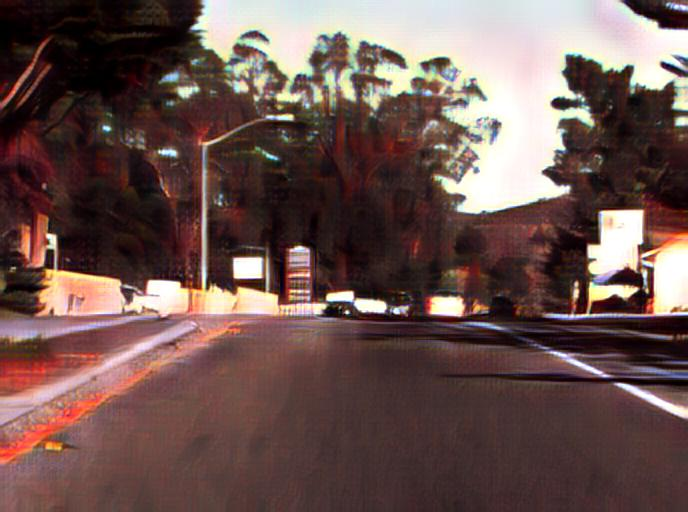
\includegraphics[width=.23\textwidth]{adin/adin1}
    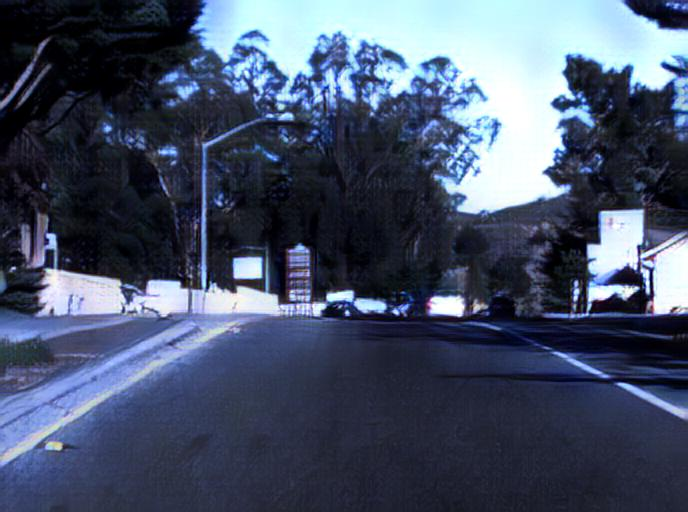
\includegraphics[width=.23\textwidth]{adin/adin2}
    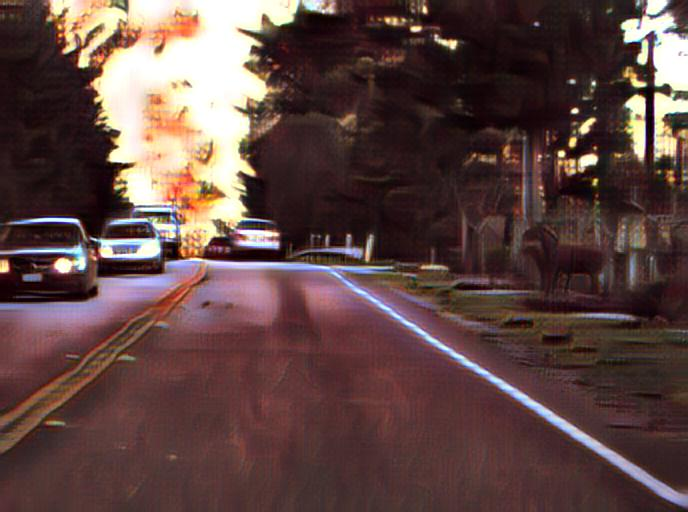
\includegraphics[width=.23\textwidth]{adin/adin3}
    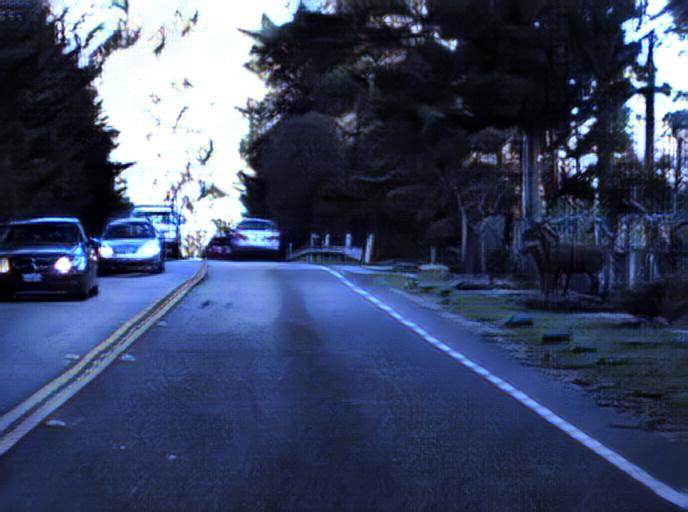
\includegraphics[width=.23\textwidth]{adin/adin4}
    \includegraphics[width=.23\textwidth]{models/adain/1}
    \includegraphics[width=.23\textwidth]{models/adain/2}
    \includegraphics[width=.23\textwidth]{models/adain/3}
    \includegraphics[width=.23\textwidth]{models/adain/4}
    \caption{AdaIN实验结果样例图}
    \label{fig:adin}
\end{figure}

% wc ~ 800

\subsubsection{Deep Photo Style Transfer}[Deep Photo Style Transfer]

\textbf{Deep Photo Style Transfer.}\cite{dpst}\quad  一般的基于Gatys等人提出的图像风格转换类似的技术都是对艺术品图像进行转换的技术,Deep Photo Style Transfer则主要针对的是显示中照片风格的转换。它主要的改进是限制了从输入图片到输出图片之间的变换为色彩空间的局部仿射变换,并且将该限制表示成了一个可自定义完全可微的能量函数。该方法可以成功地抑制合成图片中扭曲的现象。此外文献\cite{dpst}中还比较了该方法和Neural Style Transfer技术之间的转换效果,结果显示在后者出现的艺术效果以及图像中的边界扭曲效果都不存在于Deep Photo Style Transfer的合成图片中。跟之前的风格转移技术类似,也是基于将网络结构中不同层视为包含图像的内容信息和样式信息。下面简单介绍一下该技术的基本原理。

该算法不像之前的图像风格迁移技术,每次转换的输入为两组图像集合。该算法的输入仅为两张图片,与之前的一样分别为待转换的内容图片和参考的风格图片,模型的目的在于将风格图片中的风格迁移到内容图片中同时保留内容图片中的图像场景。另外该算法的一个优点是其风格图像中的Gram矩阵是基于整张图片计算的,它隐式的包含了模型中各个神经元信息,同时也限制了其分割语义图中各部分分割线的扩张。为了解决这个问题,该算法添加了为每张输入图片添加了对应的分割掩图来协助转换过程中语义分割部分转换的精确性。这些掩图被添加到原图上作为额外的通道,加上下面的分割通道来更新其风格损失函数,从而增强神经元风格算法:
\begin{equation}
    \begin{aligned}
    L_{s+}^l=\sum_{c=1}^C \frac{1}{2N_{l,c}^2}\sum_{ij}(G_{l,c}[O]-G_{l,c}[S])_{ij}^2\\
    F_{l,c}[O]=F_l[O]M_{l,c}[I]\quad F_{l,c}[S]=F_l[S]M_{l,c}[S] 
    \end{aligned}
\end{equation}
这里的$C$是语义分割掩图中的通道个数,$M_{l,c}[\cdot]$记为网络层$l$中分割掩图中的通道$c$,$G_{j,c}[\cdot]$表示对用的$F_{l,c}[\cdot]$中的Gram矩阵。为了匹配卷积神经网络中每层网络中的特征扩张空间,该算法降低了掩图的采样频率。

为了避免只出现在输入图像中的“孤独语义标记”,算法将输入的语义标记限制在了参考风格图像标记中。然而这样做可能对导致在参考样式图像上的错误标记,标记语可能在语义上大致是相同的,比如“江”和“湖”等。算法将3个部分组合形成了图像风格转换的目标函数:
\begin{align}
    L_{total}=\sum_{t=1}^L\alpha_lL_C^l+\Gamma\sum_{l=1}^L \beta_lL_{s+}^l +\lambda L_m
\end{align}
这里的$L$是卷积层的层数,$l$表示深度神经网络中的第$l$层。$\Gamma$是控制样式损失函数的权值,$\alpha_l$和$\beta_l$是调试层权重的参数。

Deep Photo Style Transfer也使用了提前训练好的VGG-19\cite{vgg-19}网络作为特征提取器,选用$conv4\_2$作为内容表征,$conv1\_1,conv2\_1,conv3\_1,conv4\_1$和$conv5\_1$作为风格表征,使用参数$\Gamma=10^2,\lambda=10^4$作为所有结果的偏好参数。

由于该模型中实现图片转换需要用到每张图片的语义分割掩图,文献\cite{dpst}中并没有给出生成掩图的代码,目前生成掩图且带有标注功能的开源工具都是基于人工对单张图片进行操作的,故而具体到我们实验的需求,对几万张Udacity数据集进行标注和语义分割,代价太大,因此我们只选用了部分数据集对该模型进行实验和结果统计。图\ref{fig:dps}是Deep Photo Style Transfer实验样例图。

\begin{figure}[h]
    \centering
    \includegraphics[width=.23\textwidth]{models/adain/1}
    \includegraphics[width=.23\textwidth]{models/adain/2}
    \includegraphics[width=.23\textwidth]{models/adain/3}
    \includegraphics[width=.23\textwidth]{models/adain/4}
    \caption{Deep Photo Style Transfer实验样例图}
    \label{fig:dps}
\end{figure}

% wc ~ 1000

\subsubsection{Fast Photo Style}[Fast Photo Style]

\textbf{Fast Photo Style.}\cite{fps}\quad  提到其他的风格转换技术中存在的问题:合成的图片往往会有不一致的风格特征,且有比较明显不真实部分。这也是该算法主要希望解决的问题。此外,算法也希望最后合成的图片应该跟用相机拍摄的照片一样真实,相较其他的主要基于色调匹配来风格化图片的技术,不同的是Fast Photo Style还关注输入图像中个内容特征的学习与提取。

\begin{figure}[t]
    \centering
    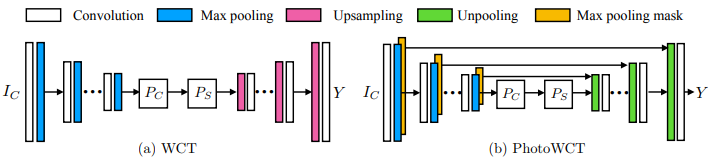
\includegraphics[width=.8\textwidth]{wct}
    \caption{}
    \label{wctf}
\end{figure}

该算法的风格化主要由两个关键步骤组成。第一步是名为PhotoWCT的样式转换$F_1$。给定一个样式图片$I_S$,$F_1$将$I_S$的风格迁移到内容图片$I_C$上,同时最小化最后的输出图片中的结构变化。虽然$F_1$可以很好的样式化$I_C$,但在语义上比较相近的区域上经常会合成样式不一致的图片。因此该算法使用了一个光滑函数$F_2$,试图借此来消除这些“坏掉的”部分。算法整体可以表达成下面的两步映射函数:
\begin{align}
    F_2(F_1(I_C,I_S),I_C)
\end{align}

PhotoWCT是基于WCT\cite{wctp}算法,为了实现真实的图片样式合成,它使用了一个新奇的网络架构。为了使用WCT,对于一般的图片重建的自动编码器被首先训练。一般的训练过程使用的是VGG-19模型作为编码器\varepsilon,并且训练解码器$D$来重建输入图片。解码器和编码器行程对称,在行为上互为逆反操作。当自动编码器训练好了,一堆映射函数就被插入到网络中,通过白化($P_C$)和彩色花($P_S$)变换来行使样式化操作。主要思想是通过两个映射函数直接将内容图像的特征相关映射到样式图片中。具体地,给定一堆内容图片$I_C$和样式图片$I_S$,首先提取除向量化的VGG特征$H_C=\varepsilon(I_C)$和$H_S=\varepsilon(I_S)$,然后再通过下面公司来转换内容特征$H_C$:
\begin{align}
    H_{CS}=P_SP_CH_C
\end{align}
这里$P_C=E_C\Lambda_C^{-\frac{1}{2}}E_C^T$,$P_S=E_S\Lambda_S^{\frac{1}{2}}E_S^T$,其中$\Lambda_C$和$\Lambda_S$是堆成三角矩阵,且有相同的协方差矩阵$H_CH_C^T$和$H_SH_S^T$。矩阵$E_C$和$E_S$是各自对用的特征向量的正交矩阵。转换后,特征方差会匹配样例图片的特征空间,即$H_{CS}H_{CS}^T=H_SH_S^T$。最后样例图片可以通过直接将转换后的特征映射到解码器$Y=D(H_{CS})$来合成。

为了解决合成图片部分区域扭曲不真实的问题,算法将原本的采样层替换成了池化层,PhotoWCT函数可以表示成:
\begin{align}
    Y=F_1(I_C,I_S)=\overline{D}(P_SP_CH_C)
\end{align}
这里的$\overline{D}$是解码器,包含了池化层的信息,用作后面的图片重构。图片\ref{wctf}展示了PhotoWCT和WCT之间的网络结构差异。

实际实现中,该算法官方给出了一个提前训练好的模型,其编码器$\varepsilon$使用了VGG-19网络结构中的conv1-1到conv4-1层,其权值由用ImageNet提前训练好的权值给定。训练数据集使用了微软COCO数据集\cite{coco}。总体来说,Fast Photo Style是一个能够实现快速合成真实图片风格转换的技术,它主要由格式化步骤和真实光滑化(photorealistic smoothing)步骤组成。该算法对上述两个步骤都给出了有效地闭环解决方案。

我们使用该模型进行了雨天、网上和雪天场景的转换,图\ref{fps-result}展示了最终实验结果样例图。
\begin{figure}[h]
    \centering
    \includegraphics[width=.23\textwidth]{fps/origin}
    \includegraphics[width=.23\textwidth]{fps/night}
    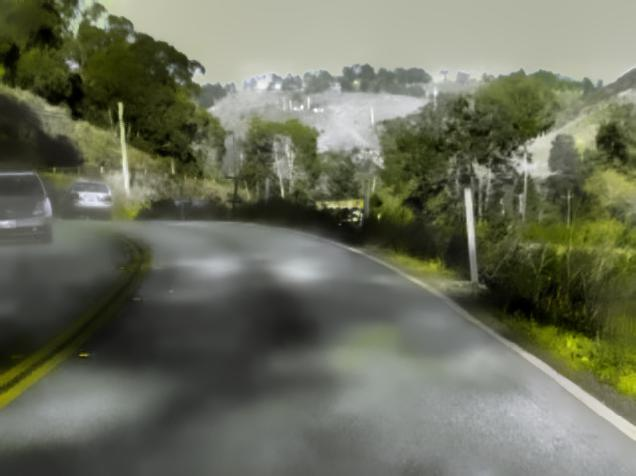
\includegraphics[width=.23\textwidth]{fps/rain}
    \includegraphics[width=.23\textwidth]{fps/snow}
    \caption{Fast Photo Style实验结果样例图}
    \label{fps-result}
\end{figure}

% wc ~ 1000
% fast photo style要求content和style image内容尽可能相近

\subsubsection{Fast Neural Transfer}

\textbf{Fast Neural Transfer.}\cite{FNT} 该算法计算单个像素的损失函数时不止考虑低层级的像素信息,还利用损失网络中的高层级特征表示的感知损失函数来训练算法的网络结构。训练过程中,感知损失能够比单个像素损失函数更好的测量出图像之间的相似度。除了图像风格的转换,Fast Neural Transfer还可用于图像的分辨率升级等应用。它通过利用感知损失函数训练的前向转换神经网络将前向图像转换任务和优化后的图像合成技术结合了起来。

该算法系统由两部分:图像转换网络$f_w$和损失网络$\Theta$。其中损失网络用来定义多个损失函数$\ell_1,\dots,\ell_k$。图像转换网络是一个由权值$W$参数化的深度残差卷积神经网络。它通过映射函数$\hat{y}=f_W(x)$将输入图片$x$转换成输出图片$\hat{y}$。每个损失函数都会计算一个标量值$\ell_i(\hat{y},y_i)$来测量输出图片$\hat{y}$和目标图片$y_i$之间的距离。该图像转换网络的训练使用了一个复杂的梯度下降算法来最小化损失函数的权值组合:
\begin{align}
    W^*=\arg \min_W E_{x,\{y_i\}}\Big[\sum_{i=1}\lambda_i\ell_i(f_W(x),y_i)\Big]
\end{align}

为了解决单个像素损失的缺点,且是损失函数更好的测量出不同图像间的语义距离,该算法使用了提前为图像分类训练好的模型。因为这些模型一般都是卷积神经网络,且都在训练阶段学习了将我们想在损失函数中测量的语义信息编码的能力。因此,算法中为了定义损失函数,选择利用提前为图像分类训练好的网络模型$\Theta$作为固定的损失网络。

对于样式转换器,其输入和输出都是像素形状为$3\times 256 \times 256$的彩色图片。对于采样因子为$f$的高清图片,其输出是像素形状为$3\times288\times288$,输入为$3\times288/f\times288/f$。因为图像转换网络是全卷积的,所以在测试阶段它们可以用于任意分辨率的图片上。

算法中提出特征重建损失值是不同特征空间中的欧几里得距离:
\begin{align}
    \ell_{feat}^{\Theta,j}(\hat{y},y)=\frac{1}{C_jH_jW_j}||\Theta_j(\hat{y})-\Theta_j(y)||_2^2
\end{align}
当输出图片与目标图片的内容差异时特征重建损失函数会惩罚输出图片,对于输入$x$,网络$\Theta$中第$j$层的激活函数记为$\Theta_j(x)$,该函数是形状为$C_j\times H_j\times W_j$的特征图谱,定义Gram矩阵为$C_j\times C_j$的方阵,其元素有下面的公式给定
\begin{align}
    G_j^{\Theta}(x)_{c,\hat{c}}=\frac{1}{C_jH_jW_j}\sum_{h=1}^{H_j}\sum_{w=1}^{W_j}\Theta_j(x)_{h,w,c}\Theta_j(x)_{h,w,\hat{c}}
\end{align}

除此之外,该算法还定义了一个简单的损失函数:像素损失函数是输出图片$\hat{y}$和目标图片$y$间的欧氏距离。如果两者的尺寸形状都为$C\times H\times W$则像素损失为$\ell_{pixel}(\hat(y),y)=||\hat{y}-y||_2^2/CHW$。图\ref{fnt-result}为该算法在我们的数据集上实验的结果样例图。

\begin{figure}[h]
    \centering
    \includegraphics[width=.23\textwidth]{FNT/origin}
    \includegraphics[width=.23\textwidth]{FNT/night}
    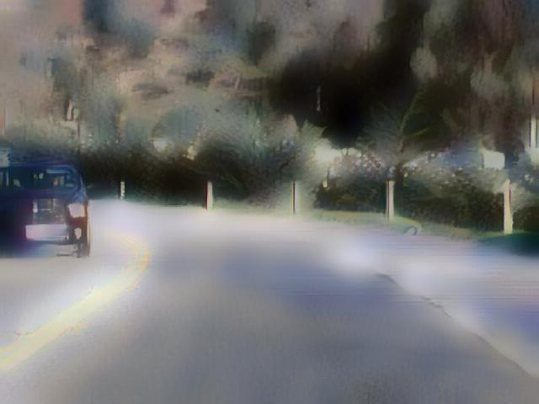
\includegraphics[width=.23\textwidth]{FNT/fog}
    \includegraphics[width=.23\textwidth]{FNT/snow}
    \caption{Fast Neural Transfer实验结果样例图}
    \label{fnt-result}
\end{figure}

\subsubsection{UDPIR} 

\newmodel{UDPIR} 该算法的主要改进点在于它提出图像逆反表示的一种方法,该方法只利用图像表征的信息,以随机噪声图片为初始值,从而可以只包含表征自身的数据信息。图像的逆反表征问题本质上是寻找一张表征与给定图像最为接近和匹配的图片,即给定表征函数$\Phi:\mathbb{R}^{H\times W\times C}\to \mathbb{R}^d$和逆反表征$\Phi_=\Phi(x_0)$,图像可通过最小化下面的目标函数实现重建:
\begin{align}
    x^*=\min_x\in \mathbb{R}^{H\times W\times C}\mathb{l}(\Phi(x),\Phi_0)+\lambda\mathb{R}(x)
\end{align}
此处的$\mathb{l}$表示重建图像的表征与给定图像表征之间的距离,文献中具体的函数使用里欧几里得距离函数:
\begin{align}
    \mathb{l}(\Phi(x),\Phi_0)=||\Phi(x)-\Phi_0||^2
\end{align}
算法的具体实现中,依然采用了提前训练好的VGG19卷积神经网络的结构来重建图像,由于文献中没有给出官方的实验代码,我们依照文献中的方法复现了MNIST数据集中数字图像的重建,但是后面试图对路况图像进行重建实验中我们发现,该算法对于数据集中$256\times 256$图片的重建合成耗时过长,约2小时一张,效率过低,因此我们放弃了对该模型的进一步实验。

\subsubsection{Targeted Style Transfer}

\newmodel{Targeted-Style-Transfer} 该算法不同之处在于只修改目标图像的某一部分而不是全部,比如只修改图片中的某一个物体而不改变物体的背景和周围场景。算法实现中除了使用了基于深度神经网络的图片修改技术还需要图像语义分割技术的协助,在物体边界的光滑化和去锯齿化中使用了马尔可夫随机场模型。

算法的具体实现是基于Gatys提出的图像风格转换技术\cite{nst},给定包含了指定风格的原图片$s$,和目标转换图片$t$,算法目标是将图像$x$转换到风格与$t$类似的新图像中,但是其中的纹理信息保留。以上可以用下面的最小方差函数表示:
\begin{align}
    \min_x ||F(x)-F(t)||^2+||C(x)-C(s)||^2
\end{align}
$F(\cdot)$是将图像映射到对应的深度特征空间的映射函数,$C(\cdot)$是将图像映射到对应特征空间协方差的映射函数。

下图\ref{fig:tst}是Targeted Style Transfer的实验样例图,如文献\cite{Targeted-Style-Transfer}提到的,该算法主要用于艺术画的图像风格转换,为了减少合成图中艺术风格的占比,我们将原模型中的VGG判别网络重新在我们的路况数据集上训练了一遍,但最后的实验结果仍不理想,图\ref{fig:tst}为最终的实验结果样例图,主要的问题是合成图的艺术画风格太重,经过实验组员讨论,决定放弃对该模型的进一步实验和数据总结。

\begin{figure}[h]
    \centering
    \includegraphics[width=.23\textwidth]{models/TST/1}
    \includegraphics[width=.23\textwidth]{models/TST/2}
    \includegraphics[width=.23\textwidth]{models/TST/3}
    \includegraphics[width=.23\textwidth]{models/TST/4}
    \caption{Targeted Style Transfer实验样例图片}
    \label{fig:tst}
\end{figure}

\subsubsection{Feedforward style transfer}

\newmodel{Feedforward-style-transfer} 该算法对于图像转换任务使用了前向转换网络,与其他算法不同的是,其损失函数不是依靠图像中的低级信息,即每个像素之间的距离,而是使用图像中的高级特征之间的距离,即感知器损失函数。模型训练过程中,感知器损失函数对图像之间的差异度量比像素见的损失函数更加可信。

该模型的主要优点是在与其他图像风格转换算法取得相似效果的同时,其模型的训练更高效。其模型训练中使用的损失函数也是创新点所在,具体训练过程使用了stochastic梯度下降算法,其损失函数为:
\begin{align}
    W^*=\min_W\mathb{E}_{x,\{y_i\}}[\sum_{i=1}\lambda_il_i(f_W(x),y_i)]
\end{align}

由于该算法跟其他的图像转换技术算法一样,主要用于艺术画的图像合成,其实验结果样例图\ref{fig:fst}如下,所以我们将该算法用在路况图像转换上,最后的合成的路况图片也都太过艺术画了,与真实场景的驾驶路况场景差距太大,因此我们放弃了该模型的进一步实验数据统计和总结。 

\begin{figure}[ht]
    \centering
    \includegraphics[width=.23\textwidth]{models/FST/1}
    \includegraphics[width=.23\textwidth]{models/FST/2}
    \includegraphics[width=.23\textwidth]{models/FST/3}
    \includegraphics[width=.23\textwidth]{models/FST/4}
    \includegraphics[width=.23\textwidth]{models/FST/5}
    \includegraphics[width=.23\textwidth]{models/FST/6}
    \includegraphics[width=.23\textwidth]{models/FST/7}
    \includegraphics[width=.23\textwidth]{models/FST/8}
    \caption{Feedforward style transfer实验结果样例图}
    \label{fig:fst}
\end{figure}

\subsubsection{Texture Nets}

\textbf{Texture Nets.}\cite{texture-nets}\quad 使用了前向生成网络来实现图像合成和风格化功能。该算法主要针对图像的纹理风格转换,文献\cite{texture-nets}中指出图片的纹理数据分布可由样本纹理数据$x_0$推导出,比如$x\sim p(x|x_0)$。在风格迁移中,分布是由图像$x_0$的视觉样式表征和另一张图片$x_1$的视觉内容表征推导出。特别的,为了从样本图片$x_0$合成纹理,这个问题可以表示为:
\begin{align}
    \min_{x\in \chi}||\Phi(x)-\Phi(x_0)||_x^2
\end{align}
对图像纹理来说,一般会假设$p(x)$是一个静态马尔科夫随机链。纹理$x_0$可以通以下公式估算局部区域的平均统计特征值:
\begin{align}
    \phi(x_0)=\frac{1}{|\Omega|}\sum_{i=1}^{|\Omega|}\psi_oF(x_0;i)\approx E_{x\sim p(x)}[\phi_oF_l(x;0)]
\end{align}

同其他的图像风格转换技术类似,该算法的损失函数也是从文献\cite{nst}中推导出来的,图像的统计数据通过固定的提前训练好的卷积神经网络(通常是VGG网络)提取出来。其Gram矩阵可以定义成一个向量矩阵和特征图谱的点积:
\begin{align}
    G_{ij}^l(x)=<F_I^l(x),F_j^l(x)>
\end{align}
因为网络属性是卷积的,所以每个点积都是所有空间特征$i$和$j$激活函数的乘积之和。模型在实际训练过程中,将Gram矩阵$G^l,l\in L_T$组合用作纹理描述表征体,这里的$L_T$包含了表征体卷积网络中卷积层的下标指数。以上可以推导除下面的图像$x$和$x_0$之间的纹理损失:
\begin{align}
    L_T(x;x_0)=\sum_{l\in L_Y}||G^l(x)-G^l(x_0)||_2^2
\end{align}
除了纹理损失函数,该算法还提出基于卷基层$l\in L_C$的输出$F_i^l(x)$来比较图片差异:
\begin{align}
    L_C(x;y)=\sum_{l\in L_C}\sum_{i=1}^{N_t}||F_i^l(x)-F_i^l(y)||_2^2
\end{align}
这里的$N_t$是第$l$层的特征通道个数。与纹理损失的主要差别在于内容损失在对应的空间区域比较特征激活函数,因此保留了空间位置信息。因此内容损失函数对于内容信息保留来说更合适,但对于纹理信息去并不合适。

算法中具体的学习过程是通过调整生成器$g(y_i,z_i;\theta)$参数$\theta$来最小化内容和纹理损失函数的组合值:
\begin{align}
    \theta_{x_o}=\min_{\theta}E_{z\sim Z;y\sim Y}[L_T(g(y,z;\theta),x_0)+\alpha L_C(g(y,z;\theta),y)]
\end{align}
这里的$Z$表示纹理合成图片的噪声分布,$y$是真实图片的实际分布,$\alpha$是平衡纹理/样式和内容的参数。图\ref{tn-example}为该模型的最终实验结果样例图以及Texture Nets官方实验结果样例图。

\begin{figure}[ht]
    \centering
    \includegraphics[width=.23\textwidth]{models/TN/1}
    \includegraphics[width=.23\textwidth]{models/TN/2}
    \includegraphics[width=.23\textwidth]{models/TN/3}
    \includegraphics[width=.23\textwidth]{models/TN/4}
    \includegraphics[width=.23\textwidth]{models/TN/5}
    \includegraphics[width=.23\textwidth]{models/TN/6}
    \includegraphics[width=.23\textwidth]{models/TN/7}
    \includegraphics[width=.23\textwidth]{models/TN/8}
    \caption{Texture Nets实验结果样例图} 
    \label{tn-example}
\end{figure}

\section{总结}

我们以文献\cite{nst-survey}为神经风格迁移技术的调研入口,初步找到了8种能够实现图像风格转换的神经风格迁移技术,即上文介绍过的AdaIN-Style,Deep Photo Style,Fast Photo Style,Fast Neural Transfer,UDPIR,Targeted Style Transfer,Feedforward Style Transfer和Texture Nets。其中Targeted Style Transfer文献\cite{Targeted-Style-Transfer}中实现的代码未开源,UDPIR文献\cite{UDPIR}中的代码由于作者放弃了维护,目前的版本不能成功运行,因此放弃了对Targeted Style Transfer和UDPIR模型的进一步实验。最终成功实验并得到数据模型有:AdaIN-Style,Deep Photo Style,Fast Photo Style,Fast Neural Transfer和Texture Nets。

\subsection{实验结果统计与分析}

\begin{figure}[h]
    \centering
    \subfigure[Fast Photo Style]{
        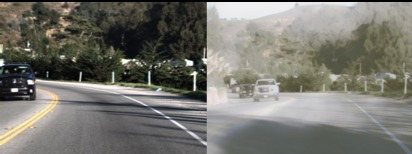
\includegraphics[width=.7\textwidth]{nst-res}
    }
    \subfigure[Fast Neural Transfer]{
        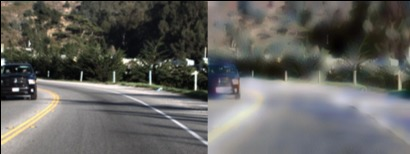
\includegraphics[width=.7\textwidth]{nst-res2}
    }
    \caption{神经风格转换技术合成图样例}
    \label{fps:sam}
\end{figure}

在得到最终实验成功的几个神经风格迁移技术的路况合成图数据后,我们对实验结果数据,即路况合成图观察后有以下2个发现:
\begin{enumerate}
    \item 神经风格迁移技术的合成图相对对抗生成网络技术的合成图而言,合成图展现的语义跟原始图十分接近,图\ref{fps:sam}第一行为Fast Photo Style对路况图像进行晴天-雾天的转换结果样例图,可以明显的看出合成图和原图在内容上表现的语义信息几乎一致。
    \item 几乎所有神经风格迁移模型的合成图都有一部分图像具有明显的艺术画风格,比如图\ref{fps:sam}第二行展示的Fast Neural Transfer的一张合成图,明显的可以看出合成图像具有艺术画特有的风格,实验的其他4中神经风格迁移技术的合成图里也有各种比例的图具有类似的艺术画风格,我们认为造成该种现象的主要原因是大部分的神经风格迁移模型的网络结构都包含了VGG-19,即他们的网络架构是相近的,导致不同的模型在训练过程中会学习到一部分类似的图像特征,从而导致不同模型最终的合成图会有大量类似的风格出现。
\end{enumerate}
